% !TeX root=../main.tex
\begin{figure}[!t]
	\hspace*{-1cm}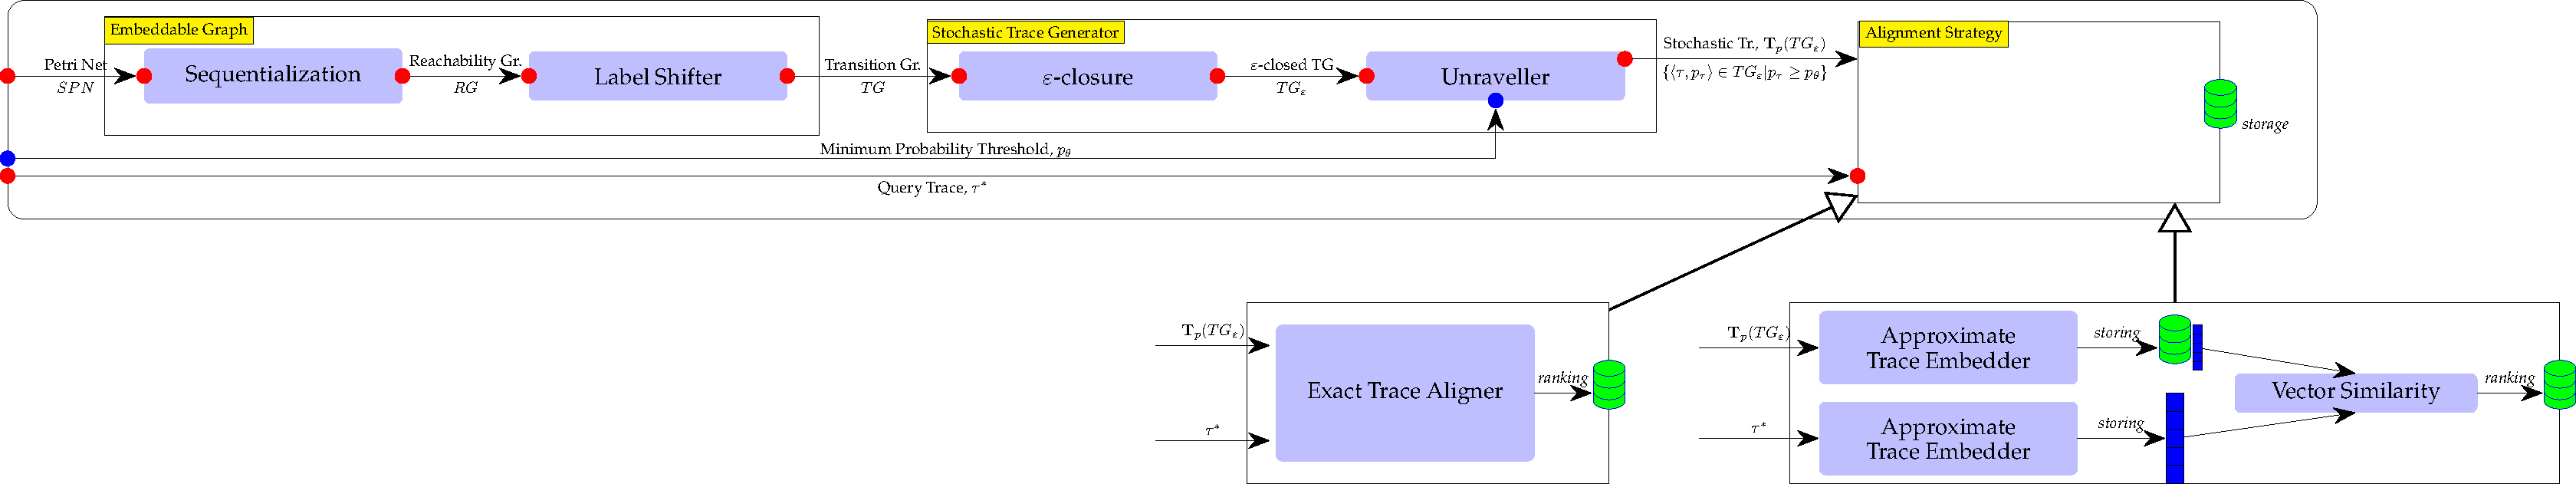
\includegraphics[width=1.2\textwidth]{images/pipeline}
	\caption{Proposed pipeline to assess the Probabilistic Trace Alignment}\label{fig:pipe}
\end{figure}


\section{Probabilistic Trace Alignment Pipeline}
We now employ the models and techniques described in Section~\ref{sec:models} to provide the main contribution of this paper, namely a technique for computing probabilistic trace alignments. More specifically, our approach takes as input 
\begin{inparaenum}[\it (i)]
\item a reference model represented as a \uswn $\net$,
\item a minimum, positive probability threshold $\pmin \in (0,1]$
\item a trace $\trace$ of interest,  
\end{inparaenum}
and returns a ranking over all the $\net$-traces having a probability greater or equal than $\pmin$, based on a combined consideration of their probability values (probabilistic component) and their distance to $\trace$ (alignment component).

\subsection{}

This is obtained through the pipeline shown in Figure~\ref{fig:pipe}, consisting of the following steps:
\begin{inparaenum}
\item the reachability graph $\rg{\net}$ of $\net$ is constructed;
\item $\rg{\net}$ is converted, by \emph{shifting labels} from transitions to states, into a corresponding transition graph $\tg_{\rg{\net}$ that preserves model traces and their probabilities;
\item the transition graph is subject to a \emph{$\hidden$-closure} that compiles away $\tau$-transitions, producing a new transition graph $\closure{\tg_{\rg{\net}}$ that preserves model traces and their probabilities while working only over visible tasks in $\tasks$;
\item this transition graph is unraveled collecting all the model traces that have a probability of at least $\pmin$;
\item we apply a probabilistic alignment technique that ranks all such model traces according to their probability and their similarity to $\trace$.
\end{inparaenum}
%
%The pipeline has the following phases: after representing the USWN as a graph of all the sequentially scheduled transitions 
%(\S\ref{sec:seqZ}), we shift the labels from the edges towards the nodes while preserving the set of probabilistic traces 
%(\S\ref{sec:LSift}) and minimize the graph representation by removing the $\tau$-labelled nodes while preserving the 
%trace probability (\S\ref{sec:clos}). 
The last step, showed as a black box in the pipeline, is realized using two alternative techniques, one more computational demanding but guaranteeing to produce an optimal ranking, the other more efficient but providing an approximate ranking.\todo{Ho tagliato la descrizione che c'era dopo. Al limite la incorporerei nella rispettiva sottosezione.}
%We later discuss how to rank traces in the exact and approximated scenarios by reducing the alignment process to a k-nearest 
%neighbour problem. While the exact trace alignment requires to perform the alignment process each time a novel trace $\sigma^*$ is 
%introduced (\S\ref{subsec:exbkptap}), the approximated alignment can split the alignment into a preliminary loading phase and a 
%query phase. In the former, each stochastic trace from the USWN is represented as a vector (\S\ref{subsec:ate}), and in the latter the to-be-aligned trace $\sigma^*$ is first represented as a vector and then compared to all the other vectorial representations.  

We now go through each step of the pipeline (but the reachability graph construction, which has been already commented).


\endinput
%
We can show that the TG obtained in Definition \ref{def:transf} preserves the same set of probabilistic traces associated by the reachability graph. The proof is omitted due to the lack of space.

\begin{example}
Figure \ref{fig:lmc} shows the TG obtained from the reachability graph in Figure \ref{fig:rg}. Nodes are labelled with the firing
transition labels (in green), and edges preserve the probabilistic information from the reachability graph (in red). Intuitively, when a
new initial node \textit{\textbf{i}} is inserted, we preserve all the initial probabilistic choices that a transition is fired from an initial
marking $M$, while the intermediate edges inherit the probabilisitc choice of the firing transition from the subsequent choices. When
a new final node \textit{\textbf{f}} is added, such edges always have probability $1$, and thus do not interfere with the
initial traces' probability.
\end{example}

\subsection{$\tau$-closure}\label{sec:clos}
The $\tau$-closure process has two main purposes: first, reduce the size of the previously generated TG by removing all
$\tau$-labelled nodes \texttt{\color{blue}w} and preserving the connection between  the nodes \texttt{\color{blue}u}
from its ingoing edges   $\texttt{\color{blue}u}\xrightarrow{\color{violet}\rho}\texttt{\color{blue}w}$ with the nodes \texttt{\color{blue}v} from its ingoing edges   $\texttt{\color{blue}w}\xrightarrow{\color{violet}\rho'}\texttt{\color{blue}v}$ by establishing new edges $\texttt{\color{blue}u}\xrightarrow{\color{violet}\rho\rho'}\texttt{\color{blue}v}$. $\tau$-labelled initial (or accepting) nodes are removed iff they have only one outgoing (ingoing) edge with probability $1$.

\begin{example}\todo{Is it now ok?}
	The $\tau$-closure removes the non-initial and non-accepting nodes within an automaton, while preserving the probabilistic trace equivalence of the two automata. Let us suppose to apply the $\tau$-closure to the automata in Figure \ref{fig:orig}: node \texttt{\color{blue}10} is removed alongside its associated edges, and new edges $\texttt{\color{blue}3}\xrightarrow{\color{violet}\rho_{65}}\texttt{\color{blue}4}$ and $\texttt{\color{blue}3}\xrightarrow{\color{violet}\rho_{6f}}\texttt{\color{blue}5}$ are introduced. The resulting TG $P$ is represented with the same graphical depiction Figure \ref{fig:closed}.
\end{example}
%
Consequently, it is always possible to minimize a TG  via $\tau$-closure, so that the only nodes labelled as $\tau$
are the source and the target nodes and the set of weighted traces is preserved. From now on, we consider only minimised TGs.

\subsection{Unraveller}\label{sec:unrav}
%Being that both the graph isomorphism problem is NP-Complete and the
Since TGs are fully characterized by the set of the probabilistic traces that they generate,  we say that two TGs are
(probabilistic-trace) equivalent iff they share the same set of weighted traces. In particular, we denote as $\mathcal{W}_p^n(P)$ the set of all the weighted traces in $P$ having at least probability $p$ and maximum length $n$. Under these assumptions, the probabilistic trace equivalence is deterministic.

\begin{example}
	The set $\mathcal{W}_0^{\aleph_0}(P^*)$ of weighted traces of the TG in Figure \ref{fig:orig} is
%	The TG in Figure \ref{fig:orig} has the following set $\mathcal{W}_0^{\aleph_0}(P^*)$ of weighted traces:
$$\set{\braket{\underbrace{\color{green}a\dots a}_{n},{\color{violet}\pa\pc^n\pf}}|n\in \mathbb{N}_{>0}}\cup \set{\braket{{\color{green}c}\underbrace{\color{green}a\dots a}_{n},{\color{violet}\pb\pd\pc^n\pf}}|n\in \mathbb{N}_{>0}}\cup\{\braket{{\color{green}cb},{\color{violet}\pb\pe}}\}$$
After the $\tau$-closure process, $\mathcal{W}_0^{\aleph_0}(P^*)=\mathcal{W}_0^{\aleph_0}(P)$, so the two TGs are (probabilistic-trace) equivalent.
\end{example}
